\documentclass[tikz,border=8pt]{standalone}
% Shared look for every TikZ diagram. Load with \input{../../tools/tikz-style.tex}
\usepackage[T1]{fontenc}
\usepackage{lmodern}
\renewcommand{\sfdefault}{lmr}  % diagrams use the same serif as the text
\usetikzlibrary{arrows.meta, positioning, shapes.geometric, calc, fit, backgrounds}
\definecolor{cblue}{HTML}{4C78A8}
\definecolor{corange}{HTML}{F58518}
\definecolor{cgreen}{HTML}{54A24B}
\definecolor{cred}{HTML}{E45756}
\definecolor{cpurple}{HTML}{B279A2}
\definecolor{cgrey}{HTML}{6B6B6B}
\tikzset{
  every picture/.style={font=\sffamily, line width=1.2pt},
  box/.style={draw=#1, fill=#1!12, rounded corners=4pt, align=center, inner sep=7pt, minimum height=1.1cm},
  box/.default=cgrey,
  arrow/.style={-{Stealth[length=3mm]}, draw=cgrey, line width=1.4pt},
  title/.style={font=\sffamily\bfseries\Large},
  note/.style={font=\sffamily\small, text=cgrey, align=center},
}
\AtBeginDocument{\hyphenpenalty=10000 \exhyphenpenalty=10000}

\begin{document}
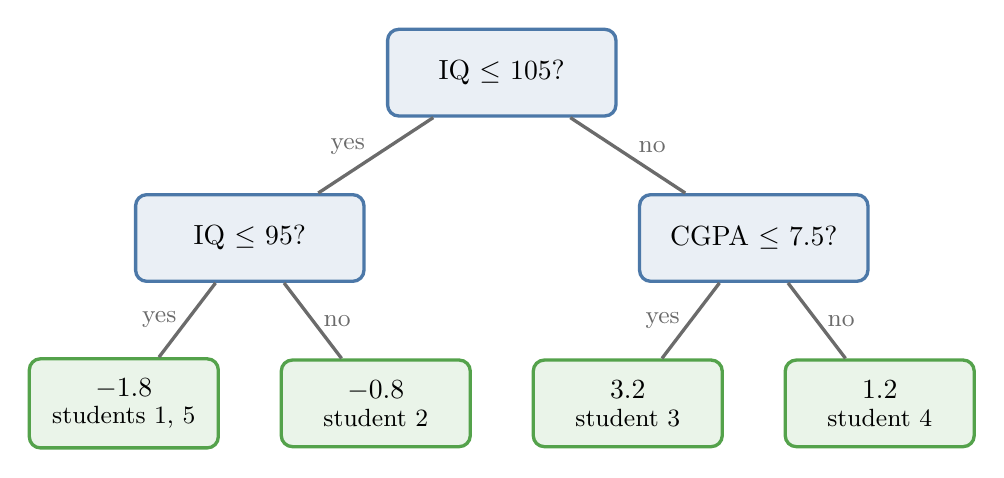
\begin{tikzpicture}[q/.style={box=cblue, minimum width=2.9cm}, l/.style={box=cgreen, minimum width=2.4cm},
  level distance=2.1cm, level 1/.style={sibling distance=6.4cm}, level 2/.style={sibling distance=3.2cm},
  edge from parent/.style={draw=cgrey, line width=1.2pt}]
  \node[q] {IQ $\le$ 105?}
    child {node[q] {IQ $\le$ 95?}
      child {node[l] {$-1.8$\\[-2pt]{\small students 1, 5}} edge from parent node[note, left] {yes}}
      child {node[l] {$-0.8$\\[-2pt]{\small student 2}} edge from parent node[note, right] {no}}
      edge from parent node[note, left, yshift=3pt] {yes}}
    child {node[q] {CGPA $\le$ 7.5?}
      child {node[l] {$3.2$\\[-2pt]{\small student 3}} edge from parent node[note, left] {yes}}
      child {node[l] {$1.2$\\[-2pt]{\small student 4}} edge from parent node[note, right] {no}}
      edge from parent node[note, right, yshift=3pt] {no}};
\end{tikzpicture}
\end{document}
